\chapter{Results}

\begin{figure}[h!]
	    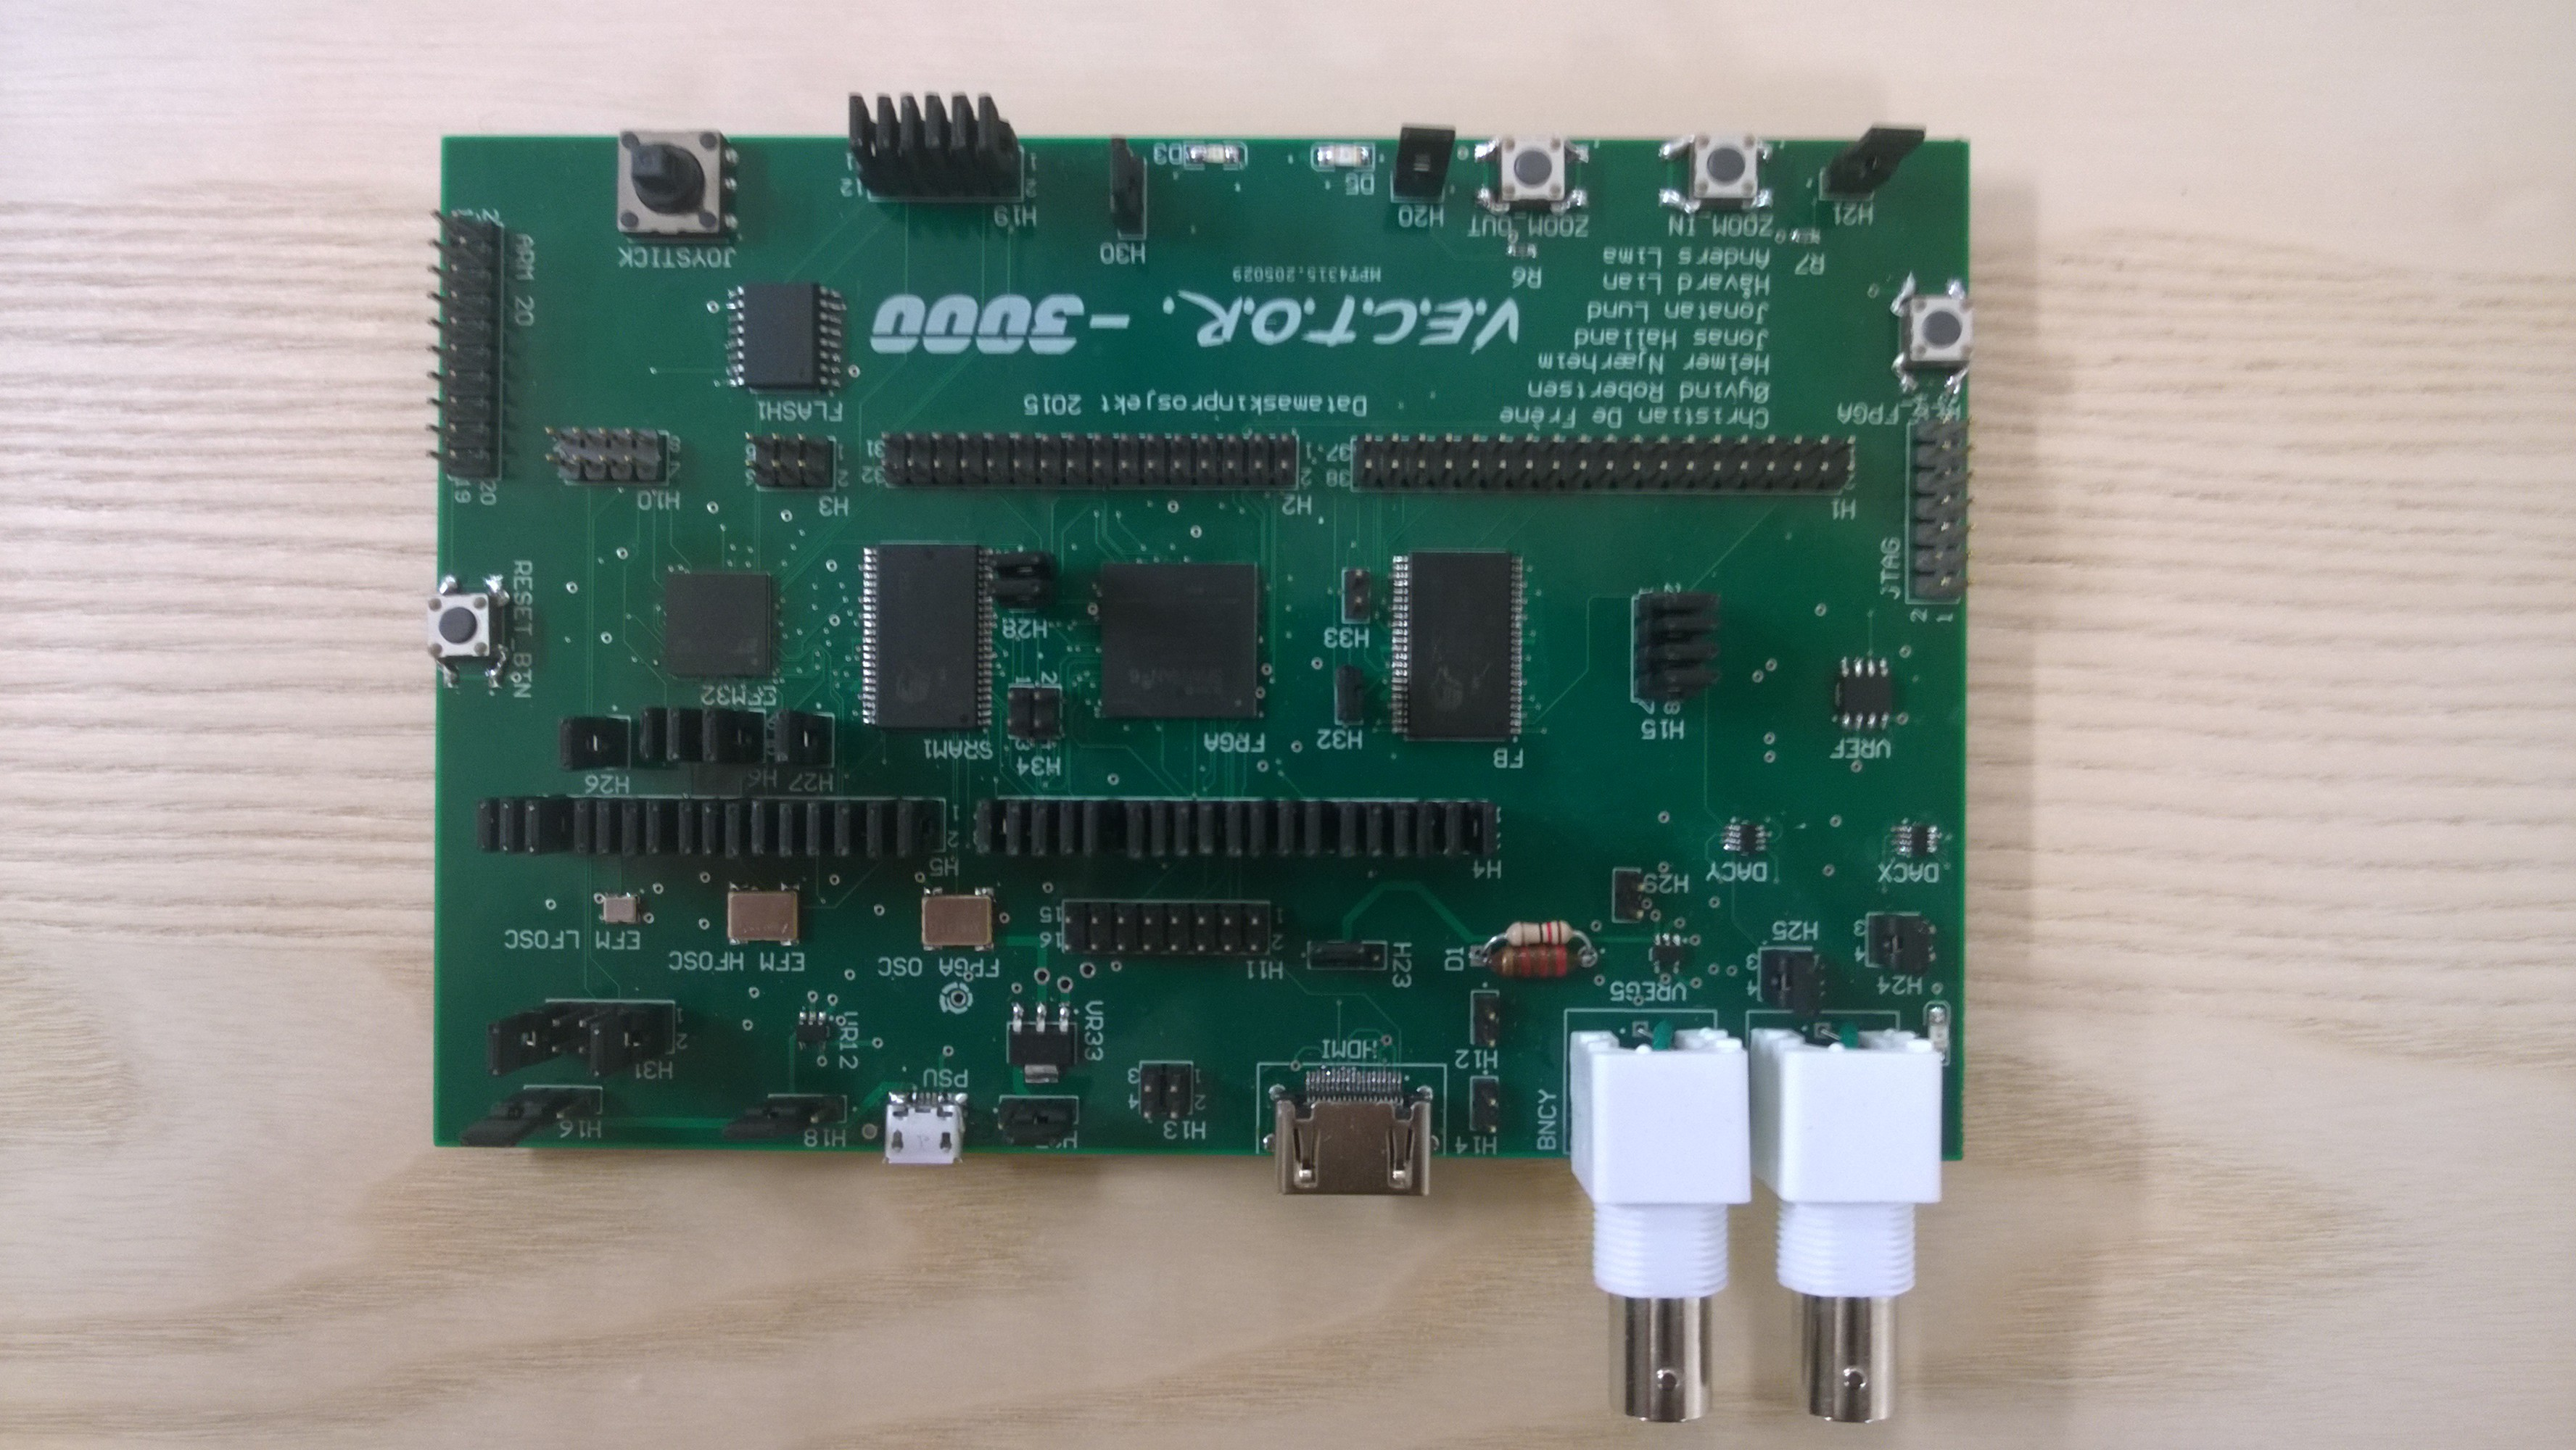
\includegraphics[width=\linewidth]{images/board.jpg}
	    \caption{An image of the finished \vthreek board}
	    \label{fig:board}
\end{figure}

\section{Storage}
The final implementation utilizes BRAM to achieve highest possible clock frequency and avoid unnecessary SRAM access delays.
With the current implementation the BRAM can hold a total of 1024 primitives.
The synthesis report from Xilinx Ise states that the FPGA still has more BRAM after.
However the primitive storage space is not the limiting factor, but the primitive drawing module.

\section{Performance}
The maximum clock frequency of the DACs is 30MHz according to the datasheet.
To update the DAC value a total of 25 clock cycles are required.
As a result the theoretical effective maximum output will be \(30 MHz \div 25 = 1.2 MHz \).
However during testing the group experience incorrect DAC values if the clock were set higher than 20 MHz.
With a clock frequency of 20 MHz the maximum output is 800 KHz.
